% 导言区,进行全局设置
\documentclass[12pt]{ctexart}%book, report, latter, 引入文档类

%\usepackage{ctex}
%\usepackage[fleqn]{amsmath}
\usepackage{amsmath}
\usepackage{amssymb}
\usepackage{fancyhdr}
\usepackage{lastpage}
\usepackage{graphicx}
\usepackage{float}
\usepackage{enumerate} % when need define format to number by myself
\usepackage[colorlinks,linkcolor=black]{hyperref} % set super link

% \newcommand命令的定义,新的命令
\newcommand\degree{^\circ}
\title{\kaishu Logistic Regression Model}
\author{Fish}
\date{\today}


% 内容与格式分离
% 设置标题的格式
\ctexset {
	section = {
		format+=\zihao {-4} \heiti \raggedright,
		name = {,},
		%number = \chinese{section},
		beforeskip = 1.0ex plus 0.2ex minus .2ex,
		afterskip = 1.0ex plus 0.2ex minus .2ex,
		aftername = \hspace{0pt}
	},
	subsection = {
		format+=\zihao{5} \heiti \raggedright,
		% name={\thesubsection},
		name = {,},
		%number = \arabic{subsection},
		beforeskip = 1.0ex plus 0.2ex minus .2ex,
		afterskip = 1.0ex plus 0.2ex minus .2ex,
		aftername = \hspace{0pt}
	}
}

% 正文区(文稿区),有且只有一个document环境
% \begim{*环境名称}
%        内容
% \end{*环境名称}
\begin{document}
	\maketitle
	%\clearpage
	\renewcommand{\contentsname}{Content} % set the 目录 to Content
	\tableofcontents
	\clearpage
	\pagestyle{fancy}
	\lhead{logistic regerssion model by wzs}                   
	\rhead{Page \thepage{} of \pageref{LastPage}}
	
	\section{\quad the exponential family}
	to work our way up to GLMs, we will begin by defining exponential family distributions. We say that a class of distributions is in the exponential family if it can be written in the form of 
	\begin{equation}
	p(y;\eta) = b(y)\text{exp}(\eta^T T(y) - a(\eta) )
	\end{equation}
	\qquad here, $\eta$ is called the natural parameter (also called the canonical parameter) of the distribution; T(y) is the sufficient statistic (for the distributions we consider, it will often be the case that T(y) = y); and $a(\eta)$ is the log partition function. The quantity $e^{-a(\eta)}$ essentially plays the role of a normalization constant, that makes sure the distribution $p(y;\eta)$ sums/integrates over y to 1.
	
	A fixed choice of T, a and b defines a family (or set) of distributions that is parameterized by $\eta$; as we vary $\eta$, we then get different distributions within this family. 
	
	we now show that the Bernouli and the Gaussian distributions are examples of exponential family distributions.
	
	\subsection{\quad Bernouli distribution}
		the Bernouli distribution with mean $\phi$, written Bernouli($\phi$), specifies a distribution over $y\in{\{0,1\}}$, so that $p(y=1;\phi) = \phi$; $p(y=0;\phi) = 1-\phi$. As we varying $\phi$, we obtain Bernouli distributions with different means. We now show that this class of Bernouli distributions, ones obtained by varying $\phi$, is in the exponential family; i.e., that there is a choice of T, a and b so that Equation (1) becomes exactly the class of Bernouli distributions.
		
		we write the Bernouli distributin as:
		\begin{align}
			\begin{split}
				p(y;\phi) &= \phi^y (1-\phi)^{1-y}\\
						  &= \text{exp}(y\log{\phi} + (1-y)\log{(1-\phi)})\\
						  &= \text{exp}((\log{(\frac{\phi}{1-\phi})})y + \log{(1-\phi)})
			\end{split}
		\end{align}
		
		thus, the natural parameter is given by $\eta = \log{(\phi/(1-\phi))}$. Interestingly, if we invert this definition for $\eta$ by solving for $\phi$ in terms of $\eta$, we obtain $\phi = \frac{1}{(1+e^{-\eta})}$. This is the familiar sigmoid function! This will come up again when we derive logistic regression as a GLM. To complete the formulation of the Bernouli distribution as an exponential family distribution, we also have 
		\begin{align}
			T(y) &= y\\
			\begin{split}
			a(\eta) &= -log(1-\phi)\\
					&= \log(1+e^\eta)
			\end{split}\\
			b(y) & = 1
		\end{align}
		
		\begin{itemize}
			\item focus on that in the process of derivation, thear is an Logistic equation
			\begin{align}
				\phi &= \frac{1}{1+e^{-\eta}} \\
				f(x) &= \frac{1}{1+e^{-x}}
			\end{align}
			
			\item sigmoid or logistic function
				\begin{figure}[H]
				\vspace{-0.2cm}  %调整图片与上文的垂直距离
				\setlength{\abovecaptionskip}{-0.2cm}   %调整图片标题与图距离
				%\setlength{\belowcaptionskip}{-1cm}   %调整图片标题与下文距离
				\centering
				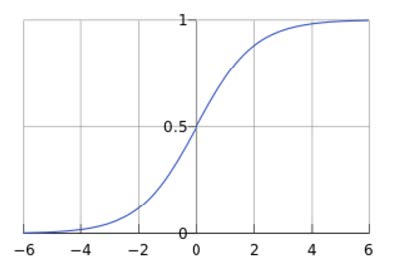
\includegraphics[scale=0.4]{sigmoid_or_logistic_function.jpg}
				\renewcommand{\figurename}{Fig} % set picture title starting with Fig or 图
				\caption{sigmoid or logistic function}
				\label{fig:1}
				\end{figure}
			
			\item derivation of sigmoid function $f(x) = \frac{1}{1+e^{-x}}$
				\begin{align}
					\begin{split}
						f'(x) &= (\frac{1}{1+e^{-x}})'\\
							  &= \frac{e^{-x}}{(1+e^{-x})^2}\\
							  &= \frac{1}{1+e^{-x}}\cdot\frac{e^{-x}}{1+e^{-x}}\\
                              &= \frac{1}{1+e^{-x}}\cdot(1-\frac{1}{1+e^{-x}})\\
						  	  &= f(x)\cdot(1-f(x))
					\end{split}
				\end{align}
		\end{itemize}
	
	\subsection{\quad Gaussian distribution}
		lets now move on to consider the Gaussian distribution. Recall that, when deriving linear regression, the value of $\sigma^2$ had no effect on our final choice of $\theta$ and $h_\theta(x)$. Thus, we can choose an arbitrary value for $\sigma^2$ without changing anything. To simlpify the derivation below, let set $\sigma^2 = 1$. We then have:
		\begin{align}
			\centering
			\begin{split}
			p(y;\mu) &= \frac{1}{\sqrt{2\pi}}e\text{x}p(-\frac{1}{2}(y-\mu)^2)\\
					 &= \frac{1}{\sqrt{2\pi}}\text{exp}(-\frac{1}{2}y^2)\cdot \text{exp}(\mu y - \frac{1}{2}\mu^2)
			\end{split}\\
			whether: \notag\\
			\eta &= \mu \notag\\
			T(y) &= y \notag\\
			a(\eta) &= \mu^2/2 \notag
					= \eta^2/2 \notag\\
			b(y) &= (1/\sqrt{2\pi})\text{exp}(-y^2/2)\notag
		\end{align}
		
	\section{\quad gradient descent algorithm(BGD SGD MBGD)}
		\begin{itemize}
			\item initialize $\theta$ (randomly initialize)
			
			\item iteration along the subtractive gradient direction, $\theta$ updated let $J(\theta)$ smaller
			\begin{equation}
				\theta = \theta - \alpha\cdot\frac{\partial J(\theta)}{\partial \theta} \qquad\alpha\text{ : learning rate、step}
			\end{equation}
			
			\item gradient descent algorithm			
				\begin{figure}[H]
					\vspace{-0.2cm}  %调整图片与上文的垂直距离
					\setlength{\abovecaptionskip}{-0.2cm}   %调整图片标题与图距离
					%\setlength{\belowcaptionskip}{-1cm}   %调整图片标题与下文距离
					\centering
					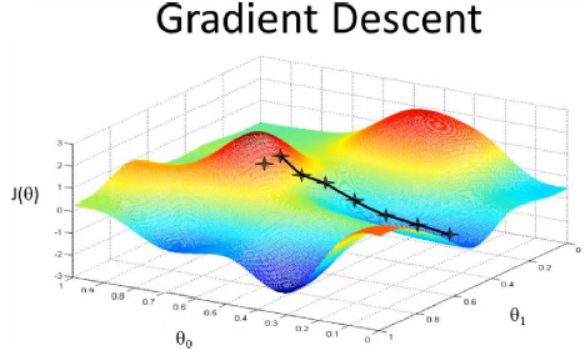
\includegraphics[scale=0.4]{gradient_descent.png}
					\renewcommand{\figurename}{Fig} % set picture title starting with Fig or 图
					\caption{gradient descent algorithm}
					\label{fig:2}
				\end{figure}
			
			\item gradient direction
				\begin{align}
					\begin{split}
						\frac{\partial}{\partial\theta_j} &= \frac{\partial}{\partial\theta_j}\frac{1}{2}(h_\theta(x) - y)^2\\
						&= 2\cdot\frac{1}{2}(h_\theta(x) - y)\cdot\frac{\partial}{\partial\theta_j}(h_\theta(x) - y)\\
						&= (h_\theta(x) - y)\cdot\frac{\partial}{\partial\theta_j}(\sum_{i=0}^{m}\theta_i x_i -y)\\
						&= (h_\theta(x) - y)x_j
					\end{split}
				\end{align}
				
			\item BGD、SGD、MBGD
		%%%%%%%%%%%%%%%%%%%%%%%%%%%%%%%%%%%%%%%%%%%%%%%%%%%%%%%%%%%%%%%%%%%%%%%%%%%%%%%%%%%%%%%%%%%%%%%
			\begin{enumerate}[(1)]
				% BGD
				%%%%%%%%%%%%%%%%%%%%%%%%%%%%%%%%%%%%%%%%%%%%%%%%%%%%%%%%%%%%%%%%%%%%%%%%%%%%%%%%%%%%%%%%%%%%%%%
				\item bach gradient descent, teh original form, mean that update gradient using all sample every iteration.
					\begin{enumerate}
						\item partial derivate target function
								\begin{equation}
									\frac{\nabla J(\theta_0, \theta_1)}{\nabla \theta_j} = \frac{1}{m}\sum_{i=1}^{m}(h_\theta(x^i) - y^i)x_j^i
								\end{equation}
								among $i = 1,2,...,m$ show sample number, $j = 0,1$ show feature number, here, we use partial part $x_0^i = 1$
								
						\item update parameter one times iteration:
								\begin{equation}
									\theta_j := \theta_j - \alpha\frac{1}{m}\sum_{i=1}{m}(h_\theta(x^i) - y^i)x_j^i
								\end{equation}
								note that here is a sum function, indicate that deal with all sample, and compare following article
								
						\item Pseudo code form as following:\\
						repeat\{
							$$\theta_j := \theta_j - \alpha\frac{1}{m}\sum_{i=1}{m}(h_\theta(x^i) - y^i)x_j^i$$
							\qquad \qquad \qquad(for $j = 0,1$)\\
						\}
						
						\item advantages:
						\begin{enumerate}
							\item calculate all sample every derivation, meanwhile operate matrix and implement parallel
							\item confirm the direction due to all dataset could represent sample population, and turn to direction fo extreme value more correctly. when target function is convex function, BGD must be able to get global optimization.
						\end{enumerate}
					
						\item disadvantages:
						\begin{enumerate}
							\item when sample number m is large, it needs calculate all sample every derivation step, and the train progress will be slow.
						\end{enumerate}
					
						\item convergence curve, that derivation number is less for it.
						\begin{figure}[H]
							\vspace{-0.2cm}  %调整图片与上文的垂直距离
							\setlength{\abovecaptionskip}{-0.2cm}   %调整图片标题与图距离
							%\setlength{\belowcaptionskip}{-1cm}   %调整图片标题与下文距离
							\centering
							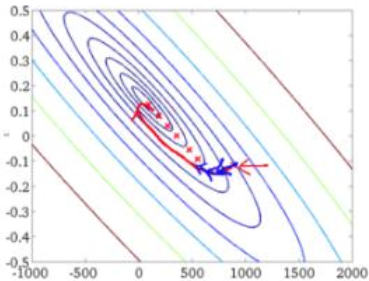
\includegraphics[scale=0.4]{Bach_Gradient_Descent.png}
							\renewcommand{\figurename}{Fig} % set picture title starting with Fig or 图
							\caption{Bach Gradient Descent}
							\label{fig:3}
						\end{figure}
					\end{enumerate}
				%%%%%%%%%%%%%%%%%%%%%%%%%%%%%%%%%%%%%%%%%%%%%%%%%%%%%%%%%%%%%%%%%%%%%%%%%%%%%%%%%%%%%%%%%%%%%%%
			
				% SGD
				%%%%%%%%%%%%%%%%%%%%%%%%%%%%%%%%%%%%%%%%%%%%%%%%%%%%%%%%%%%%%%%%%%%%%%%%%%%%%%%%%%%%%%%%%%%%%%%
				\item stochastic gradient descent, update parameter using only a sample every iteration. let train speed be accelerated.
					\begin{enumerate}
						\item target function for one sample
							\begin{equation}
								J^i (\theta_0, \theta_1) = \frac{1}{2}(h_\theta(x^i) - y^i)^2
							\end{equation}
							
						\item derivation for target function
							\begin{equation}
								\frac{\nabla J^i(\theta_0, \theta_1)}{\theta_j} = (h_\theta(x^i) - y^i)x_j^i
							\end{equation}
							
						\item parameter updated
							\begin{equation}
								\theta_j := \theta_j - \alpha(h_\theta(x^i) - y^i)x_j^i
							\end{equation}
							
						\item Pseudo code form as following:\\
						Loop\{
						
						\qquad for i = 1 to m, \{
								$$\theta_j := \theta_j - \alpha(h_\theta(x^i) - y^i)x_j^i$$
								\qquad \qquad \qquad(for $j = 0,1$)
								
						\qquad \}
						
						\}
						
						\item advantages
							\begin{enumerate}
								\item because that the loss function is not belong to the all train dataset, and in every iteration, optimize the loss function of anyone train data randomly,  it will accellerate the update speed more quickly.
							\end{enumerate}
						
						\item disadvantages
							\begin{enumerate}
								\item accuracy will be decline. although target function is convex function, SGD couldn't still converge linearly. 
								\item maybe converge to the local optimization, due to signal sample couldn't represent the trend of all sample.
								\item be not easy to realize.
							\end{enumerate}
						
						\item explain why SGD is faster than BGD for the convergence speed.\\
							answer:  here assump that it is 30W sample, one the hand, for BGD, here need calculate 30W sample every iteration and update parameter one times. So it maybe to be iterated for many times like 10 times. on the other hand, for SGD, it only needs a sample every iteration, thus when update the parameter using 30W sample, during the period, it could converge to a suitable minimize value by SGD.
							what's more, at convergence, BGD have calculated for $10\times 30W$ times, and SGD have calculated for $1\times 30W$ times. 
							
						\item convergence curve, the iteration times is pretty high, the sovelution space seem like be blind. as following:
						\begin{figure}[H]
							\vspace{-0.2cm}  %调整图片与上文的垂直距离
							\setlength{\abovecaptionskip}{-0.2cm}   %调整图片标题与图距离
							%\setlength{\belowcaptionskip}{-1cm}   %调整图片标题与下文距离
							\centering
							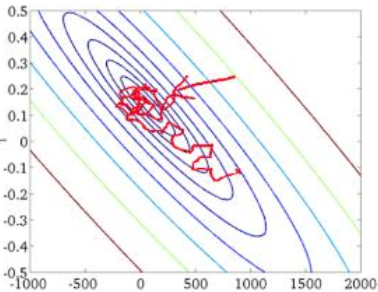
\includegraphics[scale=0.4]{Stochastic_Gradient_Descent.png}
							\renewcommand{\figurename}{Fig} % set picture title starting with Fig or 图
							\caption{Stochastic Gradient Descent}
							\label{fig:4}
						\end{figure}
					\end{enumerate}
				%%%%%%%%%%%%%%%%%%%%%%%%%%%%%%%%%%%%%%%%%%%%%%%%%%%%%%%%%%%%%%%%%%%%%%%%%%%%%%%%%%%%%%%%%%%%%%%
			
				% MBGD
				%%%%%%%%%%%%%%%%%%%%%%%%%%%%%%%%%%%%%%%%%%%%%%%%%%%%%%%%%%%%%%%%%%%%%%%%%%%%%%%%%%%%%%%%%%%%%%%	
				\item mini batch gradient descent, batch\_size sample to update parameter every iteration. here, we assump that batch\_size = 10, sample number m = 1000.
					\begin{enumerate}
						\item Pseudo code form as following:\\
							repeat\{
						
							\qquad for i = 1,11,21,31,...,991 \{
							$$\theta_j := \theta_j - \alpha\frac{1}{10}\sum_{k=i}^{i+9}(h_\theta(x^k) - y^k)x_j^k$$
							\qquad \qquad \qquad(for $j = 0,1$)
							
							\qquad \}
							
							\}
							
						\item advantages:
							\begin{enumerate}
								\item by matrix operation, optimize nenural network parameter isn't slower much than on one batch  signal data every times.
								\item it could decline iteration times enormously that converge when using one batch. meanwhile, it could make the result gotten convergence to close the impact of gradient descent.(for example, above 30W, set batch\_size = 100, need iterate for 3000 times, more less than 30W times of SGD)
								\item be able to realize parallel.
							\end{enumerate}
						
						\item disadvantages:
							\begin{enumerate}
								\item the unsuitable selection maybe bring some problem.
							\end{enumerate}
						
						\item the influence due to the selection fo batch\_size
							\begin{enumerate}[i]
								\item in reasonable range, the benefit increasing batch\_size:
									\begin{enumerate}[1)]
										\item the memory utilization rate increased, the parallel affect of big matrix multiply increased
										
										\item the iteration frequency declined when run a epoch (all dataset), for equal number of data, the calculate speed increased.
										
										\item in certain range, the more big batch\_size in general, the decline direction is preciser, the wave of train is more small.
									\end{enumerate}
								
								\item the badness of increasing batch\_size blindly
									\begin{enumerate}[1)]
										\item although the memory utilization rate increased, the capacity of memory couldn't support
										
										\item although the iteration frequency declined when run a epoch (all dataset), if want to get the equal precision, the cost time also increased, and the updated speed become slowly.
										
										\item when batch\_size increase in a certain extent, the ensure decline direction don't vary.
									\end{enumerate}
							\end{enumerate}
					\end{enumerate}
				%%%%%%%%%%%%%%%%%%%%%%%%%%%%%%%%%%%%%%%%%%%%%%%%%%%%%%%%%%%%%%%%%%%%%%%%%%%%%%%%%%%%%%%%%%%%%%%
				
				\item the picture show the convergence processing of three kind of gradient descent algorithm.
					\begin{figure}[H]
						\vspace{-0.2cm}  %调整图片与上文的垂直距离
						\setlength{\abovecaptionskip}{-0.2cm}   %调整图片标题与图距离
						%\setlength{\belowcaptionskip}{-1cm}   %调整图片标题与下文距离
						\centering
						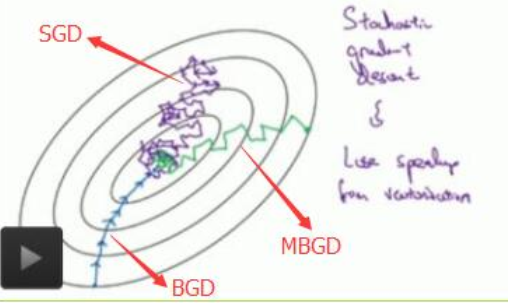
\includegraphics[scale=0.4]{Mini-Batch_Gradient_Descent.png}
						\renewcommand{\figurename}{Fig} % set picture title starting with Fig or 图
						\caption{three kinds of Gradient Descent Algorithm}
						\label{fig:5}
					\end{figure}
			\end{enumerate}
		%%%%%%%%%%%%%%%%%%%%%%%%%%%%%%%%%%%%%%%%%%%%%%%%%%%%%%%%%%%%%%%%%%%%%%%%%%%%%%%%%%%%%%%%%%%%%%%
		\end{itemize}
	
	\section{\quad logistic regression}
		\begin{enumerate}
			\item Logistic/sigmoid function\\
				you can click here to transfer that prove the sigmoid function  \url{https://www.jianshu.com/p/a8d6b40da0cf}
				\begin{align}
					\begin{split}
						h_\theta(x) &= g(\theta^T x) \\
									&= \frac{1}{1+e^{-\theta^T x}}
					\end{split}\\
					\begin{split}
						g'(x) &= (\frac{1}{1+e^{-x}})' \\
							  &= \frac{e^{-x}}{(1+e^{-x})^2}\\
							  &= \frac{1}{1+e^{-x}}\cdot\frac{e^{-x}}{1+e^{-x}}\\
							  &= \frac{1}{1+e^{-x}}\cdot(1 - \frac{1}{1+e{-x}})\\
							  &= g(x)\cdot (1-g(x))
					\end{split}\\
				\end{align}
			
			\item parameter estimate of Logistic regerssion
				\begin{enumerate}
					\item assump that :
										$$P(y=1|x;\theta) = h_\theta(x)$$
										$$p(y=0|x;\theta) = 1 - h_\theta(x)$$
										
					\item so likelihood term : $$p(y|x;\theta) = (h_\theta(x))^{y} (1-h_\theta(x))^{1-y}$$
					
					\item the likelihood function:
						  \begin{align}
						  	  \begin{split}
						  	  	  L(\theta) &= p(\vec{y}|X;\theta)\\
						  	  	  			&= \prod_{i=1}^{m}p(y^i|x^i;\theta)\\
						  	  	  			&= \prod_{i=1}^{m}(h_\theta(x^i))^{y^i} (1-h_\theta(x^i))^{1-y^i}
						  	  \end{split}
						  \end{align}
						  
					\item log likelihood function
					\begin{align}
						\begin{split}
							\ell &= \log{L(\theta)} \\
								 &= \sum_{i=1}^{m}y^i \log{h(x^i)} + (1-y^i)\log{(1 - h(x^i))}
						\end{split}\\
						\begin{split}
							\frac{\partial}{\partial \theta_j}\ell(\theta) 
							&= (y\frac{1}{g(\theta^T x)} - (1-y)\frac{1}{1-g(\theta^T x)}) \frac{\partial}{\partial\theta_j}g(\theta^T x)\\
							&= (\frac{y}{g(\theta^T x)} - \frac{1-y}{1-g(\theta^T x)}) g(\theta^T x)(1 - g(\theta^T x))\frac{\partial}{\partial\theta_j}\theta^T x\\
							&= (y(1-g(\theta^T x)) - (1-y)g(\theta^T x))x_j\\
							&= (y - h_\theta(x))x_j
						\end{split}
					\end{align}
				\end{enumerate}
			
			\item iteration of parameter
				\begin{enumerate}
					\item study rule of logistic regerssion parameter
						\begin{equation}
							\theta_j : = \theta_j + \alpha(y^i - h_\theta(x^i))x_j^i
						\end{equation}
						
					\item retult compared with the linear regression
						they have same format.
						\begin{enumerate}
							\item repeat\{
							$$\theta_j := \theta_j + \alpha\frac{1}{m}\sum_{i=1}{m}(y^i - h_\theta(x^i))x_j^i$$
							\qquad \qquad \qquad(for $j = 0,1$)\\
							\}
							
							\item 	Loop\{
							
							\qquad for i = 1 to m, \{
							$$\theta_j := \theta_j + \alpha(y^i - h_\theta(x^i))x_j^i$$
							\qquad \qquad \qquad(for $j = 0,1$)
							
							\qquad \}
							
							\}
						\end{enumerate}
				\end{enumerate}
		\end{enumerate}
	
	\section{\quad log linear model}
		\begin{enumerate}
			\item the odds fo event, indicate that the ratio between odds happen and not happen probability.
			
			\item log odds logit function
				\begin{align}
					P(y=1|x;\theta) &= h_\theta(x)\\
					P(y=0|x;\theta) &= 1 - h_\theta(x)\\
					\log it(p) 
					= \log{\frac{p}{1-p}} 
					&= \log{\frac{h_\theta(x)}{1-h_\theta(x)}} 
					= \log{\left( \frac{\frac{1}{1+e^{-\theta^Tx}}}{\frac{e^{-\theta^Tx}}{1+e{-\theta^Tx}}} \right)}
					= \theta^Tx
				\end{align} 
				
			\item loss function of logistic regression $y_i\in\{0,1\}$
				\begin{align}
					y_i&\in\{0,1\}\\
					\hat{y_i} &= \left\{
						\begin{matrix}
							p_i  &y_i = 1\\
							1-p_i   \quad &y_i=0
						\end{matrix}
						\right.\\
					L(\theta) &= \prod_{i=1}^{m}p_i^{y_i}(1-p_i)^{1-y_i} \\
					\Rightarrow \ell(\theta) &= \sum_{i=1}^{m}\ln \left[ p_i^{y_i}(1-p_i)^{1-y_i} \right]\\
					\overset{p_i = \frac{1}{1+e^{-f_i}}}{\longrightarrow} \ell{\theta} &= \sum_{i=1}^{m} \ln\left[ (\frac{1}{1 + e^{-f_i} }) ^{y_i} (\frac{1}{1+e^{f_i}})^{1-y_i}\right]\\
					\begin{split}
						\therefore loss(y_i, \hat{y_i}) &= -l(\theta)\\
														&= 	\sum_{i=1}^{m} \left[y_i\ln(1 + e^{-f_i}) + (1-y_i)\ln(1+e^{f_i})\right]
					\end{split}	
				\end{align}
				
			\item loss function of logistic regression $y_i\in\{-1,1\}$
				\begin{align}
				y_i&\in\{-1,1\}\\
				\hat{y_i} &= \left\{
				\begin{matrix}
				p_i  &y_i = 1\\
				1-p_i   \quad &y_i = -1
				\end{matrix}
				\right.\\
				L(\theta) &= \prod_{i=1}^{m}p_i^{(y_i+1)/2}(1-p_i)^{-(y_i-1)/2} \\
				\Rightarrow \ell(\theta) &= \sum_{i=1}^{m}\ln \left[ p_i^{(y_i+1)/2}(1-p_i)^{-(y_i-1)/2} \right]\\
				\overset{p_i = \frac{1}{1+e^{-f_i}}}{\longrightarrow} \ell{\theta} &= \sum_{i=1}^{m} \ln\left[ (\frac{1}{1 + e^{-f_i} }) ^{(y_i+1)/2} (\frac{1}{1+e^{f_i}})^{-(y_i-1)/2}\right]\\
				\begin{split}
				\therefore loss(y_i, \hat{y_i}) &= -l(\theta)\\
				&= 	\sum_{i=1}^{m} \left[\dfrac{1}{2}(y_i+1)\ln(1 + e^{-f_i}) - \frac{1}{2}(y_i-1)\ln(1+e^{f_i})\right]\\
				&= 
					\left\{
						\begin{matrix}
							\sum_{i=1}^{m}\left[ \ln(1+e^{-f_i})\right]   \quad &y_i = 1\\
							\sum_{i=1}^{m}\left[ \ln(1+e^{f_i})\right]    \quad &y_i = -1
						\end{matrix}
					\right.
				\end{split}	\\
				\Rightarrow loss(y_i, \hat{y_i}) &= \sum_{i=1}^{m}\left[ \ln(1+e^{-y_i \cdot f_i})\right]
				\end{align}
		\end{enumerate}
	
	\section{\quad softmax regression}
		\begin{enumerate}
			\item K classfication, the parameter of kth class  is $\vec{\theta_k}$, form two dimension matrix $\theta_{k \times n}$
			
			\item probability: 
				\begin{align}
					p(c=k|x;\theta) = \frac{\text{exp}(\theta_k^T x)}{\sum_{l=1}^{K}\text{exp}(\theta_l^T x)}, \quad k=1,2,...,K
				\end{align}
				
			\item likelihood function:
				\begin{align}
					L(\theta) = \prod_{i=1}^{m}\prod_{k=1}^{K}p(c=k|x^i; \theta)^{y_k^i} = \prod_{i=1}^{m}\prod_{k=1}^{K}\frac{\text{exp}(\theta_k^T x^i)^{y_k^i}}{\sum_{l=1}^{K}\text{exp}(\theta_l^T x^i)}
				\end{align}
				
			\item log likelihood:
				\begin{align}
					J_m(\theta) = \ln L(\theta) = \sum_{i=1}^{m}\sum_{k=1}^{K}\left( y_k^i \cdot \theta_k^T x^i - \ln \sum_{l=1}^{K}\text{exp}(\theta_l^T x^i)\right)
				\end{align}
				
			\item stochastic gradient:
				\begin{align}
					J(\theta) &= \sum_{k=1}^{K}y_k \cdot \left( \theta_k^T x - \ln \sum_{l=1}^{K} \text{exp}(\theta_l^T x)\right)\\
					\frac{\partial J(\theta)}{\partial \theta_k} &= \left( y_k - p(y_k|x;\theta) \right) \cdot x
				\end{align}
		\end{enumerate}
\end{document}